% Hopefully this will be the final version of Problem statement.
\section{Problem Statement}

% \textcolor{Maroon}{What is Cloud computing and why it is the pillar of software and other related industry. (Importance of Cloud computing.)}
% \textcolor{Maroon}{
% \begin{itemize}
% 	\item (What) The main challenge for Cloud provider is to reduce energy consumption
% 	\item WHY it is important and SO WHAT? (consequences?),
% 	\item HOW to deal with it? (Technologies)
% \end{itemize}}

\textcolor{Maroon}{Cloud computing is a practice of using a network of virtualized servers to host softwares and data \cite{Mell:2011jj}}. It provides one of the most important utilities - computation power to the modern software industry. With no upfront investment, low price and high availability (e.g 99.99\% of service time), most web service providers tend to deploy their services on Cloud. 

\textcolor{Maroon}{One of the challenges which Cloud computing has encountered, is the huge energy consumption generated by data centers} - a typical data center consumes as much energy as 25,000 households \cite{Dayarathna:2016ua}. Since energy has become the major expense of cloud providers, cutting the energy bill becomes a critical mission which will lead to a cost reduction of softwares and consequently be beneficial to most people who access the Internet on a daily basis.

\textcolor{Maroon}{To reduce the energy consumption of a data center, the main target is the physical machines (PMs) (e.g. servers).} Since among several components in a data center which consume energy such as cooling system, PMs, and network devices, PMs accounts for 40\% and have a huge improvement space, because they always run in a low utilization as observed by Barroso and Shen \cite{Barroso:2007jt,Shen:2015hm} - from 10\% to 50\% of required resources on average.

\textcolor{Maroon}{The major way to cut the energy consumption of PM is resource management \cite{Manvi:2014hm}.} Cloud resource management allocates resources to cloud users' applications, handles the workload fluctuations, and attempts to use as fewer number of PMs as possible to save energy. 

\textcolor{Maroon}{Resource management on PMs uses the \emph{virtualization} technology\cite{Uhlig:2005do}. } Virtualization can separate the resources (e.g. CPUs and RAMs) of a PM into several parts called \emph{virtual machines}, each of which runs an isolated operating system. Before virtualization technology was widely used, traditional data center assigns a PM for each application. Later on, PMs' utilization are largely improved by utilizing VMs to deploy applications. 

\textcolor{Maroon}{However, as a new trend of Service Oriented Architecture (SOA) \cite{Sprott:2004wt} appears in software industry;} SOA separates a large centralized application into multiple distributed components (e.g web services). As most of web services only require a small amount of resources,  using a VM for a web service causes resource wastage inside a VM, consequently decreasing the utilization of PMs. Therefore, a new virtualization technology: containers \cite{Felter:2015ki, Soltesz:2007cu} and a new service model: Container as a Service (CaaS) \cite{Piraghaj:2015uf} have been proposed to provide a finer granularity level of resource management. 

\textcolor{Maroon}{Container is an operating system (OS) level of virtualization which means multiple containers run on the same VM and share the OS. CaaS uses containers as the fundamental resource management units.}  That is, instead of deploying applications on VMs, applications are now deployed in containers which are running on top of VMs. This model further improves the utilization of resources as well as energy consumption \cite{Esposito:2016br}. Although this new technology gives an opportunity for better resource utilization, it also poses challenges. The challenges mainly exist in the strategy of how to place these containers in a minimum number of PMs called server consolidation \cite{Varasteh:2015fu}.

\begin{figure}
	\centering
	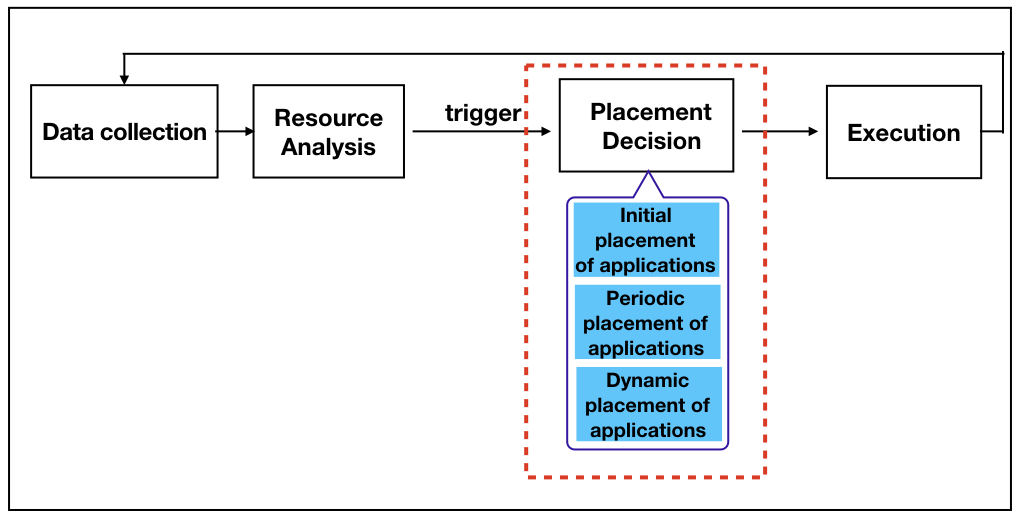
\includegraphics[width=0.7\textwidth]{pics/workflow_management.png}
	\caption{A workflow of resource management \cite{Mishra:2012kx}}
	\label{fig:workflow}
\end{figure}


\textcolor{blue}{I should illustrate the challenges in each consolidation process.}

Server consolidation optimizes the allocation of applications which has been used in three resource management scenarios: application initial placement  \cite{Jennings:2015ht}, periodic optimization \cite{Mishra:2012kx} and overloading/under-loading adjustments \cite{Mishra:2012kx} (see Figure \ref{fig:workflow}); each scenario has its unique challenges.

 % Server consumption is essentially an optimization task where it adjusts applications' locations in PMs so that a minimum number of PMs is used. For a certain number of applications, the fewer number of PMs is used, the less energy is consumed. 

% Three management processes: application initial placement, periodic optimization ,   have distinct characteristics, hence, the server consolidation techniques applied on them can be roughly classified into two categories: static \cite{Xiao:2015ik} and dynamic \cite{Beloglazov:2012bw}.

% \textcolor{Maroon}{In Initial application placement, the consolidation can be described as a static task conducted in an off-line manner.} 
\textcolor{Maroon}{To understand the challenges in each scenarios, we first describes them in a VM-based cloud.} For application initial placement, it can be seen as a static optimization task where given a number of  PMs represented as resources (e.g CPU cores and RAM etc);  a number of applications (wrapped with VMs) which also be represented as aforementioned resources; The objective is to allocate these applications into a minimum number of PMs. The decision variable is the location of each application. The basic constraint is that the aggregative resources of hosted VMs cannot exceed the PM's resource capacity.  This problem has been studied for years \cite{Xu:2010vh, Gao:2013gg, Ferdaus:2014ep} and it is often modeled as a bin packing problem \cite{Xiong:2014jq} which is NP-hard. 

\textcolor{Maroon}{In contrast, in a container-based Cloud, applications are wrapped with containers which are first allocated to a number of fixed type VMs, then, these VMs are allocated to PMs.} The decision variables are the allocation of containers to VMs and the allocation of VMs to PMs. The constraint is the demand of containers not to exceed the VM's capacity and the demand of hosted VMs not to exceed the PM's resource capacity. An additional constraint is that each container has its OS requirement which makes them cannot be simply packed into homogeneous VMs.

\textcolor{Maroon}{The major challenge for application initial placement is the two-level placement where in each level is an NP-hard problem.} In addition, these two-level placements are interact with each other, therefore, they cannot be solved separately.


% For the lower level of allocation, the objective is to maximize the utilization of resources (e.g a balanced utilization among several resources), while the upper level objective is to minimize the number of PMs. 
\textcolor{Maroon}{Periodic optimization takes existing applications' placement, re-placing them to PMs according to the nature of their workloads (e.g static, periodic or continuously changing).} Because the position of applications have been changed after this step, the live migration technique is used to move one application from one PM to another. The live migration is a very expensive operation, since it consumes network bandwidth and uses the resource on both host PM and target PM. Therefore, periodic optimization is a multi-objective task which considers minimizing the migration of applications and minimizing the overall energy consumption. 

\textcolor{Maroon}{The challenges of periodic optimization are two folds}. Firstly, it is a multi-objective task... Secondly, the variation of workload makes .... 

\textcolor{Maroon}{Overloading and underloading are scenarios which need an immediate reaction \cite{Beloglazov:2013ht}.}
Overloading is a scenario that the workloads exceed the capacity of its host PM. Hence, one or more applications will be migrated to other PMs. Underloading is when a PM runs in a low utilization, all the applications inside it will be moved to other PMs, so that the PM can be turned off. The common operation in these two scenarios are the dynamic placement \cite{Xiao:2015ik}. 

\textcolor{Maroon}{Dynamic placement places one application each time in an on-line manner.} 
In VM-based Cloud, the dynamic problem can be described as given a set of VMs and PMs, allocating these VMs to PMs iteratively so that the final solution reaches a near-optimal state.
The key point is that the migration of VM can be conducted immediately after its position is decided. Hence, essentially, the problem can be simplified to allocating one VM to PMs. The difficulty is that the iterative process is hard to reach a global optimal because it normally follows a greedy-based approach such as First Fit. In container-based Cloud,  the problem is even complicated, if no VM can accommodate a container, a new VM must be created, which incurs a second level of deployment.

\textcolor{Maroon}{The challenges of dynamic placement is also two folds.} The first challenge is the trade-off between fast reaction and global optimization \textcolor{blue}{which I should add more content later.} Second challenge is that, similar as periodic consolidation, different types of workload also need to be considered in the dynamic task, in order to match the migrated task with the existing applications in PMs. 

% Application initial placement can be seen as either static: allocate a batch of new applications, or dynamic: allocate a new application each time. In this thesis, we will consider it in both ways.

\textcolor{Maroon}{Traditional VM-based server consolidation are modeled as bin-packing problems \cite{Mann:2015ua}.}This is because VMs and PMs are naturally modeled as items and bins. Furthermore, server consolidation and bin-packing have the same optimization objective: minimize the number of bins/PMs. The complexity of bin-packing problem is NP-hard which means it is extreme time-consuming to find its optimal solution when the number of decision variables is large. However,  most research focus on VM-based server consolidation and these methods cannot be directly applied on container-based consolidation because of the different structure.

\textcolor{Maroon}{In contrast, Container-based server consolidation can be categorized as a bilevel optimization problem \cite{Colson:2007bu}.} Bilevel optimization problems contain two level of optimization task: the outer optimization task is referred as the upper level task and the inner task is referred as the lower level task. The hierarchical optimization are typically non-convex and strongly NP-hard \cite{Vicente:1994ie}. In our problem, two levels of optimization are both bin packing problems and they are cooperating.

\textcolor{Maroon}{Only few research focus on container-based server consolidation problem. One of research is from Piraghaj and et al \cite{Piraghaj:2015uf}.} They first propose a VM-resizing technique that defines the types of VM based on analyzing the historical data from Google cluster data. Then, they propose a two-step allocation: first allocate containers to VMs and then allocate VMs to PMs. They propose simple heuristics on each level of allocation, thus, did not consider the interaction between two levels (see detailed discussion in Section \ref{container-based-placement}). In addition, they propose a dynamic placement \cite{Piraghaj:2016bw} using a series simple heuristics such as Random Host Selection Algorithm or First Fit Host Selection. Their resource allocation system completely relies on dynamic placement without using static methods. Although their system can execute allocation fast, the energy efficiency cannot be guaranteed. Another research  \cite{Mann:2016hx} is the earliest study which realizes when deploying applications or containers, the VM size selection and VM placement should be considered together because they are interact with each other. They apply a fixed VM placement algorithm and considering a series of VM selection algorithms such as simple selection \cite{Ganesan:2012eb},  Multiple selection, Maxsize, Consolidation-friendly. The results also proves that the interaction between two placement cannot be ignore. Their resource allocation system completely relies on dynamic placement without using static methods. Although their system can execute allocation fast, the energy efficiency cannot be guaranteed. Another research  \cite{Mann:2016hx} is the earliest study which realizes when deploying applications or containers, the VM size selection and VM placement should be considered together because they are interact with each other. They apply a fixed VM placement algorithm and considering a series of VM selection algorithms such as simple selection \cite{Ganesan:2012eb},  Multiple selection, Maxsize, Consolidation-friendly. The results also proves that the interaction between two placement cannot be ignored.

\textcolor{Maroon}{Furthermore, for periodic optimization problem, most research only consider static workload \cite{} which is a simplified assumption.} According to Fehling \cite{Fehling:2014tl}, applications' workload are roughly classified into five categories: static, periodic, once-in-a-life-time, continuously changing, and unpredictable. Current studies either considers workload as static which remains constant throughout its life cycles, or \textcolor{blue}{Find some Refs deal the workload as a whole.} Only a few research consider applying different strategies on different workloads. Meng et al \cite{Meng:2010gh} use a time-series analysis on workloads; they mapped complementary periodic workload as pairs and allocate them together. Their experiments showed promising results, however, they only mapped paired workloads which is unrealistic in practice.

\textcolor{Maroon}{In addition, dynamic placement is often addressed use simple bin-packing heuristic such as First Fit, Best Fit Decreasing \cite{} and manually designed heuristics.} Simple bin-packing heuristic often cannot provide good performance because, as Mann's research \cite{Mann:2015ua} showed, server consolidation is a lot harder than bin-packing problem because of the multi-dimensional of resources, heterogeneous PMs, migration cost etc. Therefore, general bin-packing algorithms do not perform well.\textcolor{blue}{Discussed the disadvantage of human design heuristics.}




%  Secondly, they use a two-step allocation. Because of the interaction of two allocations, separated optimization approach will lead to local optima \cite{Mann:2016hx}. Therefore, these two allocations should be considered simultaneously.




The overall goal of this thesis is to develop new container-based server consolidation approaches to solve three problems: joint allocation of containers  and VMs, periodic global optimization and dynamic placement. 
